\documentclass{umemoria}

\usepackage{lipsum}
\usepackage[utf8]{inputenc}
\usepackage[acronym, toc]{glossaries}
\usepackage[fixlanguage]{babelbib}
\usepackage{url}
\usepackage[T1]{fontenc}
\usepackage{import}
\usepackage{hyperref}

\makeglossaries

\depto{Departamento de Ciencias de la Computación}
\author{Marcelo Esteban Becerra Alarcón}
\title{Mejora de un sistema de mesa de ayuda para estudiantes del DCC}

\memoria{Ingeniero Civil en Computación}

\guia{Jocelyn Simmonds} 

\comision{}

\begin{document}

\frontmatter
\maketitle


\newglossaryentry{latex}
{
    name=latex,
    description={Is a mark up language specially suited for scientific documents}
}

\newacronym{cadcc}{CADCC}{Centro de Alumnos del Departamento de Ciencias de la Computación}

\newacronym{dcc}{DCC}{Departamento de Ciencias de la Computación, de la Universidad de Chile}

\newacronym{ps}{CC5402}{CC5402 Proyecto de software} 

\newacronym{e}{CC6908}{CC6908 Introducción al trabajo de título}

\newacronym{f1}{CC6909}{CC6909 Trabajo de Titulo}

\newacronym{f2}{CC6910}{CC6910 Trabajo de Memoria de Titulo}

\newacronym{S}{\textit{Alumno S}}{alumno auto suficiente}

\newacronym{R}{\textit{Alumno R}}{alumno regular}

\newacronym{P}{\textit{Alumno P}}{alumno práctico}

\newacronym{UCD}{UCD}{User Centered Desing}

\newacronym{f}{FG}{\textit{Focus Group}}

\newglossaryentry{i*}{
    name=i*,
    description={El lenguaje de modelamiento i*, fue introducido como un marco de referencia orientado a modelar actores y objetivos. Consiste en un lenguaje de modelamiento junto con una serie de tecnicas que permiten analizar estos modelos. \cite{Dalpiaz2016}}
    }
    
\newglossaryentry{effectiveGUI}{
    name=Efective GUI,
    description= {Cuando se habla de \textit{Efective GUI} o interfaz gráfica efectiva para el usuario, se habla de una interfaz que está diseñada para simular o reemplazar una interacción humana, se acuña principalmente en el área de IA relacionada con los chatbots}
    }

\newglossaryentry{Telegram}{
    name=Telegram,
    description= {Telegram es un software gratiuto, multiplataforma, basado en la nube, de mensajería instantanea. El servicio además provee video encriptado de principio a fin, VoIP, envío de archivos y varias otras funciones. Fue lanzado para iOS en Agosto 14 2013 y Android en Octubre 2013 }
}

\newglossaryentry{Celery}{
    name=Celery,
    description= {Telegram es un software gratiuto, multiplataforma, basado en la nube, de mensajería instantanea. El servicio además provee video encriptado de principio a fin, VoIP, envío de archivos y varias otras funciones. Fue lanzado para iOS en Agosto 14 2013 y Android en Octubre 2013 }
}

\newglossaryentry{Django}{
    name=Django,
    description= {Telegram es un software gratiuto, multiplataforma, basado en la nube, de mensajería instantanea. El servicio además provee video encriptado de principio a fin, VoIP, envío de archivos y varias otras funciones. Fue lanzado para iOS en Agosto 14 2013 y Android en Octubre 2013 }
}

\newglossaryentry{ORM}{
    name=ORM,
    description= {Telegram es un software gratiuto, multiplataforma, basado en la nube, de mensajería instantanea. El servicio además provee video encriptado de principio a fin, VoIP, envío de archivos y varias otras funciones. Fue lanzado para iOS en Agosto 14 2013 y Android en Octubre 2013 }
}

\newglossaryentry{ODM}{
    name=ODM,
    description= {Telegram es un software gratiuto, multiplataforma, basado en la nube, de mensajería instantanea. El servicio además provee video encriptado de principio a fin, VoIP, envío de archivos y varias otras funciones. Fue lanzado para iOS en Agosto 14 2013 y Android en Octubre 2013 }
}

\newglossaryentry{REST}{
    name=REST,
    description={Representational State Transfer, architectural style for distributed hypermedia systems}
}
 % opcional

\begin{resumen}
   \par El \acrfull{dcc}, ha tenido un aumento sustancial en la cantidad de alumnos que ingresan a la carrera. Esto implica que se generen una serie de desafíos en torno a los procesos académicos. Estos desafíos generan un aumento en la carga de los funcionarios y docentes, a su vez que hacen que no se pueda responder con la velocidad necesaria que requieren los cambios. Esto aumenta la incertidumbre por parte de los alumnos, sobre todo en la forma de abordar los diferentes desafíos de los procesos académicos. Este proyecto busca continuar la extensión de un sistema de mesa de ayuda, pensado para modernizar el trato efectivo entre alumnos, profesores y funcionarios. Mejorando su infraestructura y añadiendo funcionalidades clave para la continuidad y mejora del proyecto.

   \par Este proyecto se realizó en 4 fases. En primer lugar, se efectuó un nuevo levantamiento de datos para evaluar la percepción de los alumnos del sistema actual, y adquirir nociones que permitieran hacer un diseño centrado en el usuario de las nuevas funcionalidades. A partir de estos resultados se integraron los objetivos y preferencias de los alumnos de manera explícita en el sistema, y se agruparon en categorías funcionales y cualitativas las valoraciones de los alumnos.

   \par Luego se hizo un proceso de diseño de alto nivel a través del lenguaje de modelación \gls{i*}. Este se traspasó a un diseño basado en casos de uso a través de \acrshort{uml}. Finalmente, se produjo un diseño de funcionalidades de 3 partes que contempla: las preferencias y objetivos de los usuarios, las opciones en el sistema y, las funcionalidades específicas que permiten dar cumplimento a las dichas alternativas.

   \par Después, se procedió a un proceso de análisis y reestructuración del código actual, lo que permitió añadir nuevas funcionalidades, así como mejorar el sistema existente, asegurando su extensibilidad. Se solucionaron problemas de compatibilidad y \textit{bugs} en el código.

   \par Finalmente, se implementaron nuevas tecnologías como \textit{\gls{Celery}}, que permitieron la implementación de funcionalidades de suscripción personalizada. Permitiendo a cada alumno agregar recordatorios de los procesos habilitados.

   \par Este trabajo extiende las funcionalidades anteriores y reestructura el código existente, de manera de crear un sistema extensible y personalizable, favoreciendo la continuidad de este servicio. Logrando así los objetivos planificados.
   
\end{resumen}
\begin{dedicatoria}
    Una dedicatoria corta.
\end{dedicatoria}
\begin{thanks}
      
    Quiero agradecer a varias personas, porque el que esté aquí en este preciso momento, es gracias a muchas, muchas almas, que dedicaron tiempo, amor, conocimiento y paciencia para mí.

    \par A mis Padres: Porque fueron el sustento de todo mi aprendizaje y de mis ganas de ir más lejos. Que me inculcaron el amor por el conocimiento y la sabiduría más allá de mis estudios.

    \par A mi esposa: Que se ha convertido en mi tesoro, mi partner, mi idónea, mi igual, que ha llenado de dicha incluso aquellos días de cansancio extremo. Porque gracias a su amor he crecido, he sanado y vuelto a encantarme de mí mismo y he encontrado nueva belleza en la vida.

    \par A mis hermanas: Que han sido mis grandes compañeras hasta este momento dónde por fin se ha cerrado una primera gran, gran etapa de aprendizaje. Las quiero mucho.

    \par A mis abuelos Ramón, Marta y Lola: Que siempre creyeron y han creído en mí. Que se han deleitado con todos mis logros. Cuya lucha y esfuerzo, más la misericordia divina nos ha permitido vivir una vida llena de amor, a pesar, de que ustedes mismos no recibieron una vida así.

    \par A toda mi familia: Que a pesar de nuestros errores y diferencias, se siguen amando y siguen estando el uno para el otro.

    \par Al PCM: Por ser una antorcha en mi camino, por haber despertado un nuevo amor por todos los seres humanos. Por todo el saber que han compartido y por ser unos increíbles \guillemotleft ñoños\guillemotright, unos excelentes amigos y por traer a Dios de forma constante a mi vida en los momentos más densos del estudio.

    \par A todos mis amigos: Por darme tantas perspectivas diferentes a la mía y ser un cable a tierra en mis \guillemotleft ñoñerías\guillemotright, por sentarse a disfrutar conmigo durante toda esta etapa universitaria.

    \par A todos mis profesores: Que con tanto esfuerzo y dedicación me llenaron de energía, curiosidad y cariño por el aprendizaje. Un especial saludo a las tías del jardín que no ven este final, pero que le confiaron sus laboriosas horas a ese pequeñito que no sabía aún escribir. Y también a la profesora Jocelyn que me ha acompañado en todo este proceso de titulación, por su paciencia y muchos consejos.

\end{thanks}
% \section{Estado del Arte}
    \par Para el desarrollo de este trabajo se hizo una investigación sobre los sistemas que solucionan problemas similares y a que objetivos responden. Al mismo tiempo como abordar el hecho de que el usuario es parte fundamental del flujo del sistema tanto en su funcionamiento como imponiendo restricciones dinámicas sobre el mismo, las que responderían a preferencias o valores de cada usuario. Por este motivo los temas abordados a continuación son \textit{\acrfull{UCD}}, \textit{human in the loop}, \textit{information systems} y \textit{chatbots}.
    
    \subsection{User centered desing - privacy, cutomization and confiability}
    \par Este es un sistema que indudablemente se basa en el usuario y sus preferencias, es por esta razón que para que el desarrollo sea exitoso no basta con que se desarrolle de la manera correcta y asumiendo buenas prácticas, sino que debe hacerse en torno al usuario y rescatando no sólo su input \cite{Karat1997}, sino sus objetivos y valores. Dentro de las maneras de enfocar un desarrollo centrado en el usuario encontramos 3 alternativas la especialista, generalista y mixto \cite{Fox2008}.
    \par la manera especialista hace referencia a que hay 3 actores encargados del proceso, los usuarios, los encargados de \acrshort{UCD} y el resto del equipo de desarrollo. Por otro lado, la generalista asume dos roles: el de usuario y el de desarrollador encargado de esta área.
    \par En esta línea de \textit{\acrlong{UCD}}, el diseño propiamente tal, se entiende como un proceso, en el que debe estar involucrado el usuario final, de forma constante.
    De modo que la personalización llega a ser "una pieza fundamental del diseño exitoso es aterrizar el desarrollo de \textit{features} y herramientas sobre el valor del usuario final" \cite{Kramer2000}.
    \par De aquí se obtiene que el sistema debería ser personalizable, y rescatar lo que sea valorado por los usuarios. Dada la naturaleza del proyecto, se decide adoptar un enfoque generalista.
    
    \subsection{Information Sistem and Human in the loop}
    \par Al ser un sistema que depende del usuario para determinar el curso de acción, el humano en este sistema no solo está en ciertos momentos críticos del flujo, sino que es el centro del flujo de información, modelos como este han sido validados con buenos resultados \cite{Smith2018} recientemente.
    \par Los sistemas de información asociados a chatbots, generalmente buscan la integración de información, este proceso es decir mostrarle al usuario una gran variedad de información de diferentes fuentes a través de una vista unificada viene asociado a varias dificultades técnicas y teóricas \cite{Li2017}.
    \par En este sentido, se propone que los sistemas de información que dependen de un humano son altamente complejos, porque los humanos, en este caso usuarios no solo son observadores, sino que tienen la capacidad de incidir en el ambiente no solo reaccionar al ambiente \cite{McBride2021}, sería iluso desarrollar un sistema para las personas sin considerar los objetivos de ellas de forma explícita en el diseño del sistema.
    \par Estos descubrimientos e investigaciones ponen varias restricciones en cuanto al desarrollo de un sistema que depende los usuarios para funcionar y que al mismo tiempo está centrado en el usuario. Pero las podemos condensar en al menos 2: El diseño del sistema debe considerar de forma explícita los objetivos del usuario en cada interacción y debe integrar la información.
    \subsection{Chabots}
    \par Los chatbots se utilizan desde hace varios años para variados y diversos fines, en múltiples áreas. En particular ahora los abordaremos desde la esfera académica, centrándonos específicamente en instituciones de educación superior.
    En estas se utilizan principalmente como un medio de apoyo al proceso de aprendizaje, como soporte para procesos universitarios, como ayuda para la gestión académica y cómo un sistema de consulta que responde a dudas de diversos entes de estas instituciones.
    
    \par Como apoyo al proceso de aprendizaje los chatbots se han usado tanto dentro como fuera de la sala de clases.
    \par En la \textit{University of Salerno}, se creó un sistema para responder de manera efectiva las preguntas de los estudiantes, el contexto de \textit{e-learning}. A grandes rasgos es un sistema que usa procesamiento de lenguaje natural como técnicas de ontología, para ligar las preguntas de los estudiantes al contenido disponible y de esta forma poder responder eso que los alumnos están buscando \cite{Clarizia2018}
    \par El Dr. Sherif Abdelhamid del \textit{Virginia Polytechnic Institute and State University} también propuso un sistema de características similares \cite{Abdelhamid2020}, con las distinciones de que uso el sistema de reconocimiento de voz para traducir las dudas verbales de los estudiantes a texto y así procesarlas y que su objetivo estaba ligados a los elementos que acompañaban al estudio más que al aprendizaje académico en sí. Algunos ejemplos como cuál es la bibliografía pertinente al curso, que recursos tiene disponibles, que debería aprender, etc.
    \par En este aspecto, investigadores del \textit{Department of Mathematics and Computer Science, University of Kabianga, Kericho, Kenya} con miembros del \textit{Department of Curriculum Instruction Educational Media, School of Education, Moi University, Kenya} analizaron la respuesta de los mismos profesores a la introducción de estas herramientas en la rutina de enseñanza \cite{K2018}
    
    \par Como soporte para procesos universitarios los chatbots se han usado para entregar el horario de clases o las clases siguientes así cómo ayudar a los alumnos a elegir ramos.
    
    \par Desarrolladores de la \textit{Bogdan Khmelnytsky Melitopol State Pedagogical University} en Ucrania, desarrollaron un servicio de 3 capas para poder implementar un servicio de ayuda al entregar el horario de clases a través de un chatbot, esto se hacía no solo con la finalidad de ayudar a alumnos que hayan olvidado o no un horario o su sala, sino también porque los horarios pueden sufrir cambios o modificaciones, además de que si bien hay alternativas simples como fotos estas se pierden en un gran volumen de elementos similares sin relación, lo que las hace difícil de volver a obtener, según la investigación. \cite{Priadko2019}
    
    \par En \textit{The Open University of Hong Kong Hong Kong} desarrolladores implementaron un sistema para facilitar a los alumnos la decisión sobre qué cursos tomar a través de un chatbot \cite{ChunHo2018}.
    
    \par En el área de los desarrollos de ayuda para la gestión académica, se encontraron desarrollos ligados a: Hacer disponibles servicios en horarios no hábiles, Mantener, monitorear y mostrar la información del alumno y Acercar la implementación de chatbots a usuarios de más alto nivel y con menos conocimiento técnico.
    
    \par Los trabajos de Vaishnavi Ajay Inamdar1 y Shivanand R.D en el \textit{BIET College} de la India, van enfocados en poder proveer servicios de gestión académica en cualquier momento, de este modo bajar la carga de los funcionarios y proveer de una \textit{\gls{effectiveGUI}} \cite{Journal2019}
    
    \par Del \textit{Engineering Rajalakshmi Institute of Technology} una profesora y sus alumnos, desarrollaron un sistema para administrar la información escolar de los alumnos y está ligado la base de datos de administración. Este sistema tenía el foco en el personal administrativo de la institución y dependía de la información entregada por el alumno.
    
    \par Con el foco en los apoderados o tutores de un alumno, en la \textit{Universitas Komputer Indonesia} A Heryandi, desarrolló un sistema de chatbots para poder desplegar las notas y el rendimiento de los alumnos a los padres usualmente menos versados en tecnología y más familiarizados con plataformas de mensajería. Por esto mismo se desarrolló un sistema con \textit{Easy access}, es decir, con un login o un proceso de autenticación sencillo y con información conocida por los tutores \cite{Heryandi2020}.
    
    \par En Indonesia en la \textit{Universitas Sebelas Maret} investigadores desarrollaron un sistema con un bot de Telegram para incluir a funcionarios no expertos en el diseño de funcionalidades para la universidad. Este proveía funcionalidades como agregar botones, comandos, acciones, mensajes directos, transmitir mensajes, configuraciones y análisis \cite{Hasyim_2021}.
    
    \par Como un sistema de consulta se han desarrollado sistemas de preguntas frecuentes, algunos ejemplos son el sistema de Mesa de ayuda del DCC \cite{ARANCIBIA2021} y un trabajo de la \textit{Manipal University} en la India \cite{Ranoliya2017}.
    \par Aunque ambos son similares, responden a necesidades completamente distintas, el sistema del DCC es un proyecto centrado en el usuario, mientras que el trabajo de la India tiene un foco en la performance y el uso de IA.
    
    \subsection{Análisis de las soluciones actuales}
    \par Como se puede observar los bots cumplen variadas funciones dentro de la vida universitaria a través del mundo, apoyando a toda la comunidad escolar, tanto tutores, como funcionarios y alumnos, haciendo más accesibles, disponibles y eficientes diversos servicios, incluso apoyando procesos de aprendizaje virtual y presencial.
    \par A pesar de la gran diversidad de funcionalidades que están presentes en estos sistemas, se logra rescatar que en la mayoría de los casos se diseña basándose en un modelo de inputs, procesamiento y respuestas. En la mayoría de los casos a pesar de ser desarrollos que buscan acercar o facilitar la vida de sus usuarios, suelen tomar un enfoque técnico y centrarse en aspectos como tener una \textit{\acrshort{effectiveGUI}}, son desarrollos que en general carecen de un modelo que integre al usuario directamente, y se enfocan en solucionar los problemas de manera analítica o teórica. Esto podría ser una enorme dificultad para el proyecto e iría en contra de los descubrimientos en el área de \textit{\acrlong{UCD}}.
    \par Por estas razones se opta por tomar los buenos resultados funcionales de los chatbots, pero agregarles de alguna forma las preferencias de los usuarios de forma explícita en el diseño de los nuevos modelos de interacción.


\tableofcontents
\listoftables % opcional
\listoffigures % opcional

\mainmatter

% \chapter{Introducción}

\lipsum[30-35]
\begin{enumerate}
	\item Item 1
	\begin{enumerate}
		\item Subitem 1
		\item Subitem 2 (ver Figura \ref{logofcfm})
	\end{enumerate}
	\item Item 2
	\item Item 3
\end{enumerate}
\begin{teo}
Se tiene que $$\int_0^t e^sds=e^t-1.$$
\end{teo}
\lipsum[36-40]
% \chapter{Segundo}

\lipsum[1-3]

\begin{defn}[ver \cite{KAR00}] Definición definitiva $$\frac{d}{dx}\int_a^xf(y)dy=f(x).$$\end{defn}
% \chapter{Tercero}
\lipsum[50-60]
% \chapter{Conclusión}

\lipsum[130-132]
\begin{figure}
	\centering
	
\includegraphics[scale=.2]{imagenes/fcfm.pdf}
	\caption{Logo de la Facultad}
	\label{logofcfm}
\end{figure}

\lipsum[133-134]

\begin{table}
	\centering
	\caption{Tabla 1}
	\label{tabla:1}
	\begin{tabular}{|c|c|r|}
		\hline
		\textbf{Campo 1} & \textbf{Campo 2} & \textbf{Num} \\\hline
		Valor 1a & Valor 2a & 3\\
		Valor 1b & Valor 2b & 3\\
		\hline
	\end{tabular}

\end{table}

\lipsum[135]


% ver https://www.overleaf.com/learn/latex/Glossaries




\printglossaries[type=\acronymtype]
\printglossaries

\nocite{*}
\bibliographystyle{babplain}
\bibliography{bibliografia}

\newpage
\begin{appendices}
    \chapter*{Anexo}
\end{appendices}

\begin{figure}[h]
    \centering
    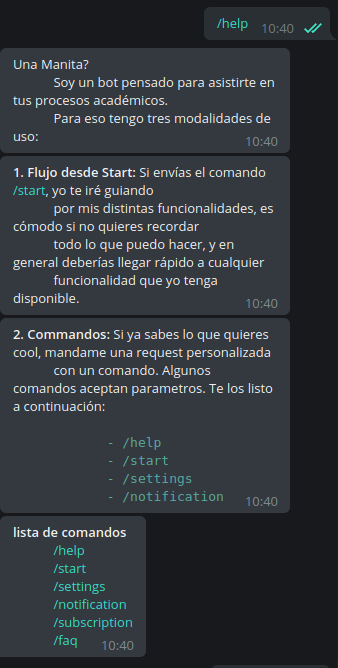
\includegraphics[scale=0.5]{media/imagenes/sc/help.png}
    \caption[Bot help]{Captura de pantalla del Bot Respondiendo el nuevo comando help}
\end{figure}

\end{document}
